\documentclass[style=gt,mode=present,paper=screen]{powerdot}
\pdsetup{%
	logohook=tl,logopos={0.02\slideheight,0.98\slideheight},
	logocmd={
\includegraphics[height=0.09\slideheight]{GT.eps}}}
\title{The AXIN Protocol}
\author{Dan Gisselquist, Ph.D.}
\date{\today}
%
% Mail to orconf@fossi-foundation.org, and slides will be taken care of
%
%
% \usepackage[dvips]{draftcopy}
% \draftcopySetGrey{0.9}
% \draftcopyName{DRAFT}{135}
\usepackage{fvcharts}
\usepackage[normalem]{ulem}
\usepackage{bytefield}
\usepackage{tikz-timing}
\usetikztiminglibrary[rising arrows]{clockarrows}
\usepackage{enumitem}
\definecolor{dkblue}{rgb}{0,0,0.6}
% \hypersetup{pdftitle={\thetitle}}
% \hypersetup{pdfauthor={\theauthor}}
\definecolor{waveletgray}{gray}{0.85}
\definecolor{inputclr}{rgb}{0,0.5,0.5}
\newcommand{\zhref}[2]{\href{#1}{\textcolor{dkblue}{#2}}}
\begin{document}


\begin{emptyslide}{}
\begin{pspicture}(0,0)(\slidewidth,0.6\slidewidth)
	% \psframe(0,0)(\slidewidth,0.6\slidewidth)%
\rput[bl](0.04\slidewidth,-0.064\slidewidth){
\rput(0.2\slidewidth,0.325\slidewidth){% semin = 0.08\slidewidth
\rput(0.025\slidewidth,0.04\slidewidth){
\includegraphics[width=0.41\slidewidth]{gfx/GT.eps}}
\rput[lt](-0.18\slidewidth,-0.11\slidewidth){\parbox{3.5in}{\fontfamily{cmr}\selectfont\Huge Gisselquist\\[-0.012\slidewidth]Technology, LLC}}%
	\rput(-0.18\slidewidth,-0.256\slidewidth){
		\rput(0,0){\psline[linecolor=barblue,linewidth=0.06in]{-}%
			(0,0)(0.6\slidewidth,0)}%
		\rput(0.73\slidewidth,0){\psplot[%
			plotpoints=5000,linewidth=0.06in,%
			plotstyle=line,linecolor=barblue]{-2.5}{1.75}{
			dup abs 30 lt {
				dup 60 div
				dup 180 mul cos
					dup dup mul mul
					0.45 mul exch
				180 mul 8 mul sin
				mul
				1.5 mul
			} { 0 } ifelse }}
	}
}
\rput(0.685\slidewidth,0.3\slidewidth){\makebox(0,0){\scalebox{1.5}{\parbox{0.272\slidewidth}{\begin{center}%
		\fontfamily{cmr}\selectfont\large Building Generic Bus Properties
		\end{center}}}}}
% 1.5 * boxwidth should be 3.5
\rput(0.69\slidewidth,0.183\slidewidth){\makebox(0,0){\scalebox{1.5}{\parbox{0.24\slidewidth}{% 
		\fontfamily{cmr}\selectfont\tiny%
		Daniel~E.~Gisselquist,~Ph.D.\\
		March, 2023}}}}
}\end{pspicture}\end{emptyslide}
%

\section{AXIN Protocol}
%
\begin{slide}[method=file]{Signals}
\begin{tabular}{c||c|c|}
Global & AXI & AXIN \\
Signals & Stream &\\\hline\hline
\textcolor{inputclr}{\tt ACLK} & \textcolor{inputclr}{\tt TVALID} & \textcolor{inputclr}{\tt VALID} \\
\textcolor{inputclr}{\tt ARESETN}  & {\tt TREADY} & {\tt READY} \\\hline\hline
               & \textcolor{inputclr}{\tt TDATA}  & \textcolor{inputclr}{\tt DATA} \\
               & \textcolor{inputclr}{\tt TSTRB}  & \textcolor{inputclr}{\tt BYTES} \\
               & \textcolor{inputclr}{\tt TKEEP}  & \\
               & \textcolor{inputclr}{\tt TLAST}  & \textcolor{inputclr}{\tt LAST} \\
               &                                  & \textcolor{inputclr}{\tt ABORT} \\
               & \textcolor{inputclr}{\tt TUSER}  & \\\hline
\end{tabular}

\hbox{}\rput[tb](0,0){%
	\onslide{2-3}{%
	\rput(0.75in,0.30in){\psline[linecolor=red,linewidth=2\pslinewidth,framearc=0.1](0,0)(0.6in,0in)}%
	\rput(0.75in,0.88in){\psline[linecolor=red,linewidth=2\pslinewidth,framearc=0.1](0,0)(0.6in,0in)}%
	\rput(0.75in,1.06in){\psline[linecolor=red,linewidth=2\pslinewidth,framearc=0.1](0,0)(0.6in,0in)}%
	}\onslide{2}{%
	\rput*[l](0,-0.05in){\psframebox[linecolor=red,linewidth=2\pslinewidth,framearc=0.1]{\textcolor{red}{\Large These signals arean't really needed}}}}%
	\onslide{3}{%
	\rput(1.4in,0.4in){\psframe[linecolor=dkgreen,linewidth=2\pslinewidth,framearc=0.1](0,0)(0.55in,0.2in)}
	\rput(1.4in,0.97in){\psframe[linecolor=dkgreen,linewidth=2\pslinewidth,framearc=0.1](0,0)(0.55in,0.2in)}
	\rput*[l](0,-0.05in){\psframebox[linecolor=dkgreen,linewidth=2\pslinewidth,framearc=0.1]{\parbox{2.5in}{\textcolor{dkgreen}{\Large We'll add these two new ones}}}}}
}
\end{slide}
%
%
\begin{slide}[method=file]{ABORT}
\begin{enumerate}
\item ABORT may be raised at any time
\end{enumerate}
\begin{tikztimingtable}[%
  timing/dslope=0.1,
  timing/.style={x=3ex,y=2ex},
  x=5ex,
  timing/rowdist=3ex
]
\textcolor{inputclr}{ACLK}      & 19{c} \\
\textcolor{inputclr}{VALID}   &  1l L 7H 1L \\
READY    & 1l 4H 3L H 1L \\
\textcolor{inputclr}{DATA}    &  1l L D{} D{} D{} 4D{} 1L \\
\textcolor{inputclr}{ABORT}   &  1l L 5L 2H 1L \\
\end{tikztimingtable}\rput(0,0){%
	% \rput(-1in,0.5in){\psline[linecolor=dkgreen,linewidth=2\pslinewidth](0,0)(0.42in,0)}
	% \rput(-1in,0.3in){\psline[linecolor=dkgreen,linewidth=2\pslinewidth](0,0)(0.4in,0)}
	% \rput(-1in,0.10in){\psline[linecolor=dkgreen,linewidth=2\pslinewidth](0,0)(0.4in,0)}
}

It may be raised while \zinline{VALID && !READY}.
\end{slide}
%
%
\begin{slide}[method=file]{ABORT}
\begin{enumerate}
\item ABORT may be raised at any time
\end{enumerate}
\begin{tikztimingtable}[%
  timing/dslope=0.1,
  timing/.style={x=3ex,y=2ex},
  x=5ex,
  timing/rowdist=3ex
]
\textcolor{inputclr}{ACLK}      & 19{c} \\
\textcolor{inputclr}{VALID}   &  1l L 4H 4L \\
READY    & 1l 5H 3L 1L \\
\textcolor{inputclr}{DATA}    &  1l L D{} D{} D{} D{} 4U \\
\textcolor{inputclr}{ABORT}   &  1l L 6L 1H 1L \\
\end{tikztimingtable}\rput(0,0){%
	% \rput(-1in,0.5in){\psline[linecolor=dkgreen,linewidth=2\pslinewidth](0,0)(0.42in,0)}
	% \rput(-1in,0.3in){\psline[linecolor=dkgreen,linewidth=2\pslinewidth](0,0)(0.4in,0)}
	% \rput(-1in,0.10in){\psline[linecolor=dkgreen,linewidth=2\pslinewidth](0,0)(0.4in,0)}
}

It may be raised even without raising \zinline{VALID}.
\end{slide}
%
%
\begin{slide}[method=file]{ABORT}
\begin{enumerate}
\item ABORT may be raised at any time
\item ABORT may be only be released if not stalled
\end{enumerate}
\begin{tikztimingtable}[%
  timing/dslope=0.1,
  timing/.style={x=3ex,y=2ex},
  x=5ex,
  timing/rowdist=3ex
]
\textcolor{inputclr}{ACLK}      & 19{c} \\
\textcolor{inputclr}{VALID}   &  1l L 7H 1L \\
READY    & 1l 4H 3L H 1L \\
\textcolor{inputclr}{DATA}    &  1l L D{} D{} D{} 4D{} 1L \\
\textcolor{inputclr}{ABORT}   &  1l L 4L 3H 1L \\
\end{tikztimingtable}\rput(0,0){%
	% \rput(-1in,0.5in){\psline[linecolor=dkgreen,linewidth=2\pslinewidth](0,0)(0.42in,0)}
	% \rput(-1in,0.3in){\psline[linecolor=dkgreen,linewidth=2\pslinewidth](0,0)(0.4in,0)}
	% \rput(-1in,0.10in){\psline[linecolor=dkgreen,linewidth=2\pslinewidth](0,0)(0.4in,0)}
}

% It may be raised even without raising \zinline{VALID}.
\begin{zformal}
property assert (@(posedge ACLK)
        disable iff (!ARESETN)
        (VALID && !READY && ABORT)
                |=> VALID && ABORT);
\end{zformal}
\end{slide}
%
%
\begin{slide}[method=file]{ABORT}
\begin{enumerate}
\item ABORT may be raised at any time
\item ABORT may be only be released if not stalled
\item While legal, it doesn't make sense to raise ABORT if \zinline{VALID && LAST}.
\item \onslide{2}{Nor does it make sense to raise ABORT if a packet hasn't started.}
\end{enumerate}
\begin{tikztimingtable}[%
  timing/dslope=0.1,
  timing/.style={x=3ex,y=2ex},
  x=5ex,
  timing/rowdist=3ex
]
\textcolor{inputclr}{ACLK}      & 19{c} \\
\textcolor{inputclr}{VALID}   &  1l L 5H 3L \\
READY    & 1l 4H L 4H \\
\textcolor{inputclr}{DATA}    &  1u U D{} D{} D{} 2D{} 3U \\
\textcolor{inputclr}{LAST}    &  1l L 3L 2H 3L \\
\textcolor{inputclr}{ABORT}   &  1l L 4L H L H 1L \\
\end{tikztimingtable}\rput(0,0){%
	\rput(-0.7in,0.1in){\psellipse[linecolor=red,linewidth=2\pslinewidth](0.16in,0.16in)}%
	\rput(-0.3in,0.1in){\onslide{2}{\psellipse[linecolor=red,linewidth=2\pslinewidth](0.16in,0.16in)}}
	% \rput(-1in,0.3in){\psline[linecolor=dkgreen,linewidth=2\pslinewidth](0,0)(0.4in,0)}
	% \rput(-1in,0.10in){\psline[linecolor=dkgreen,linewidth=2\pslinewidth](0,0)(0.4in,0)}
}

If \zinline{VALID && LAST} are both true, the packet has
successfully, entered the downstream registers.  Raising ABORT
at this point makes little sense.
\end{slide}
%
%
\begin{slide}[method=file]{BYTES}
\begin{enumerate}
\item All beats are packed
\item The BYTES field contains \zinline{$clog2(DW/8)} bits.

	If ever \zinline{BYTES == 0}, then there are
	\zinline{DW/8} valid bytes implied.

\item Only the last beat can contain fewer than DW/8 bytes
\item The last beat cannot be empty.  It must have at least one byte.
\item Ordering can be big \onslide{2}{or little} endian
\end{enumerate}

\begin{center}
\onslide{1}{\rput[t](0,0){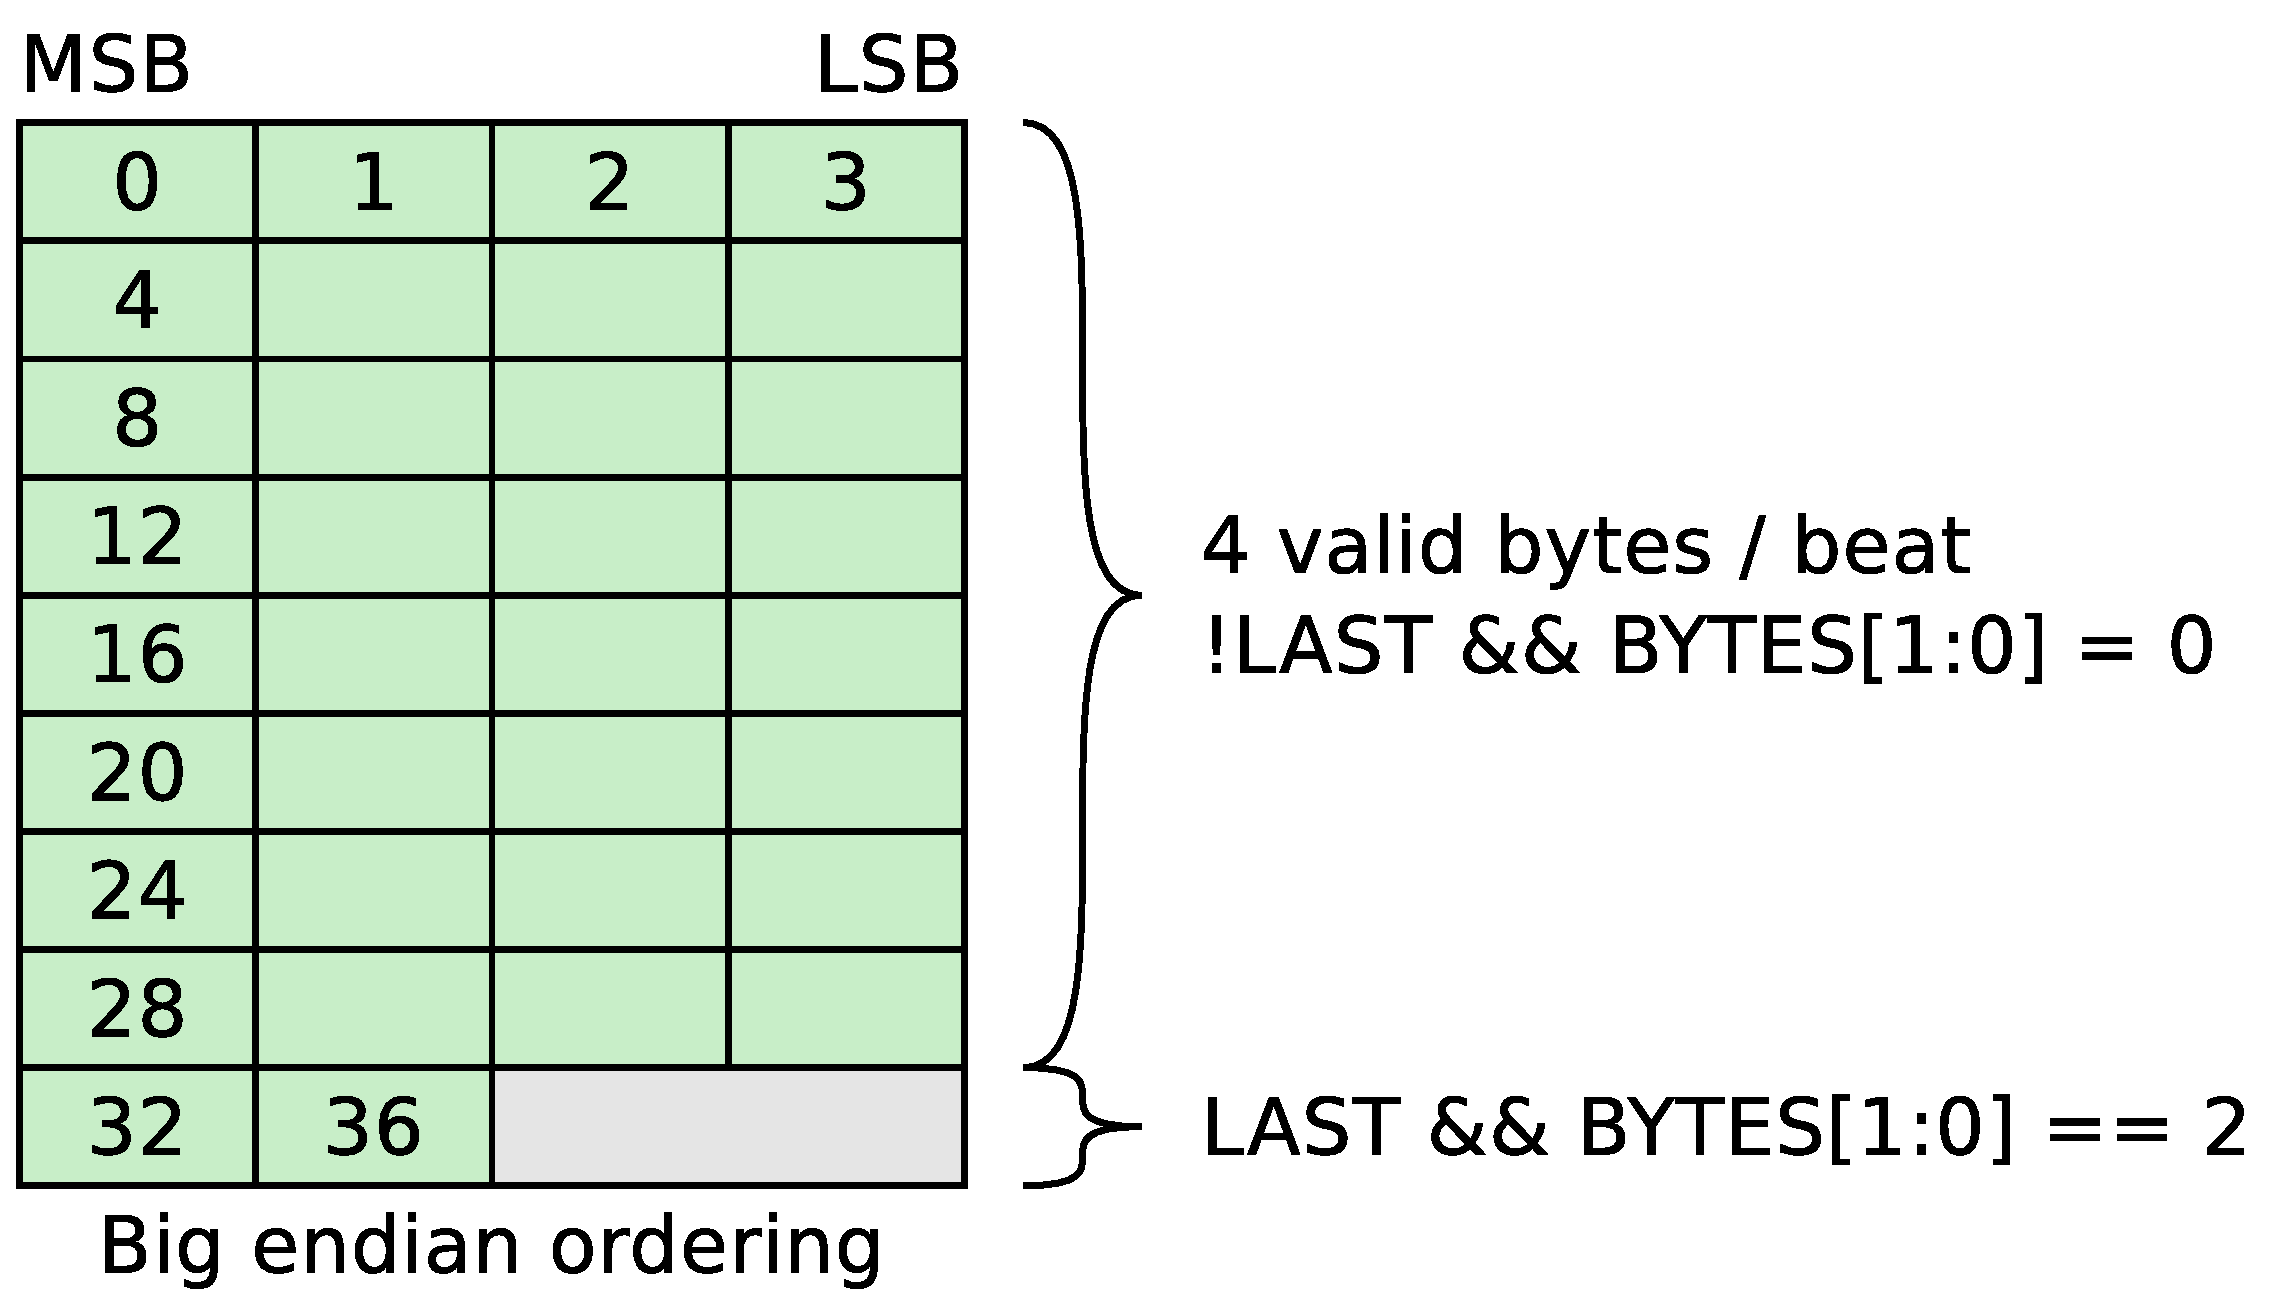
\includegraphics[width=2in]{big-endian.eps}}}%
\onslide{2}{\rput[t](0,0){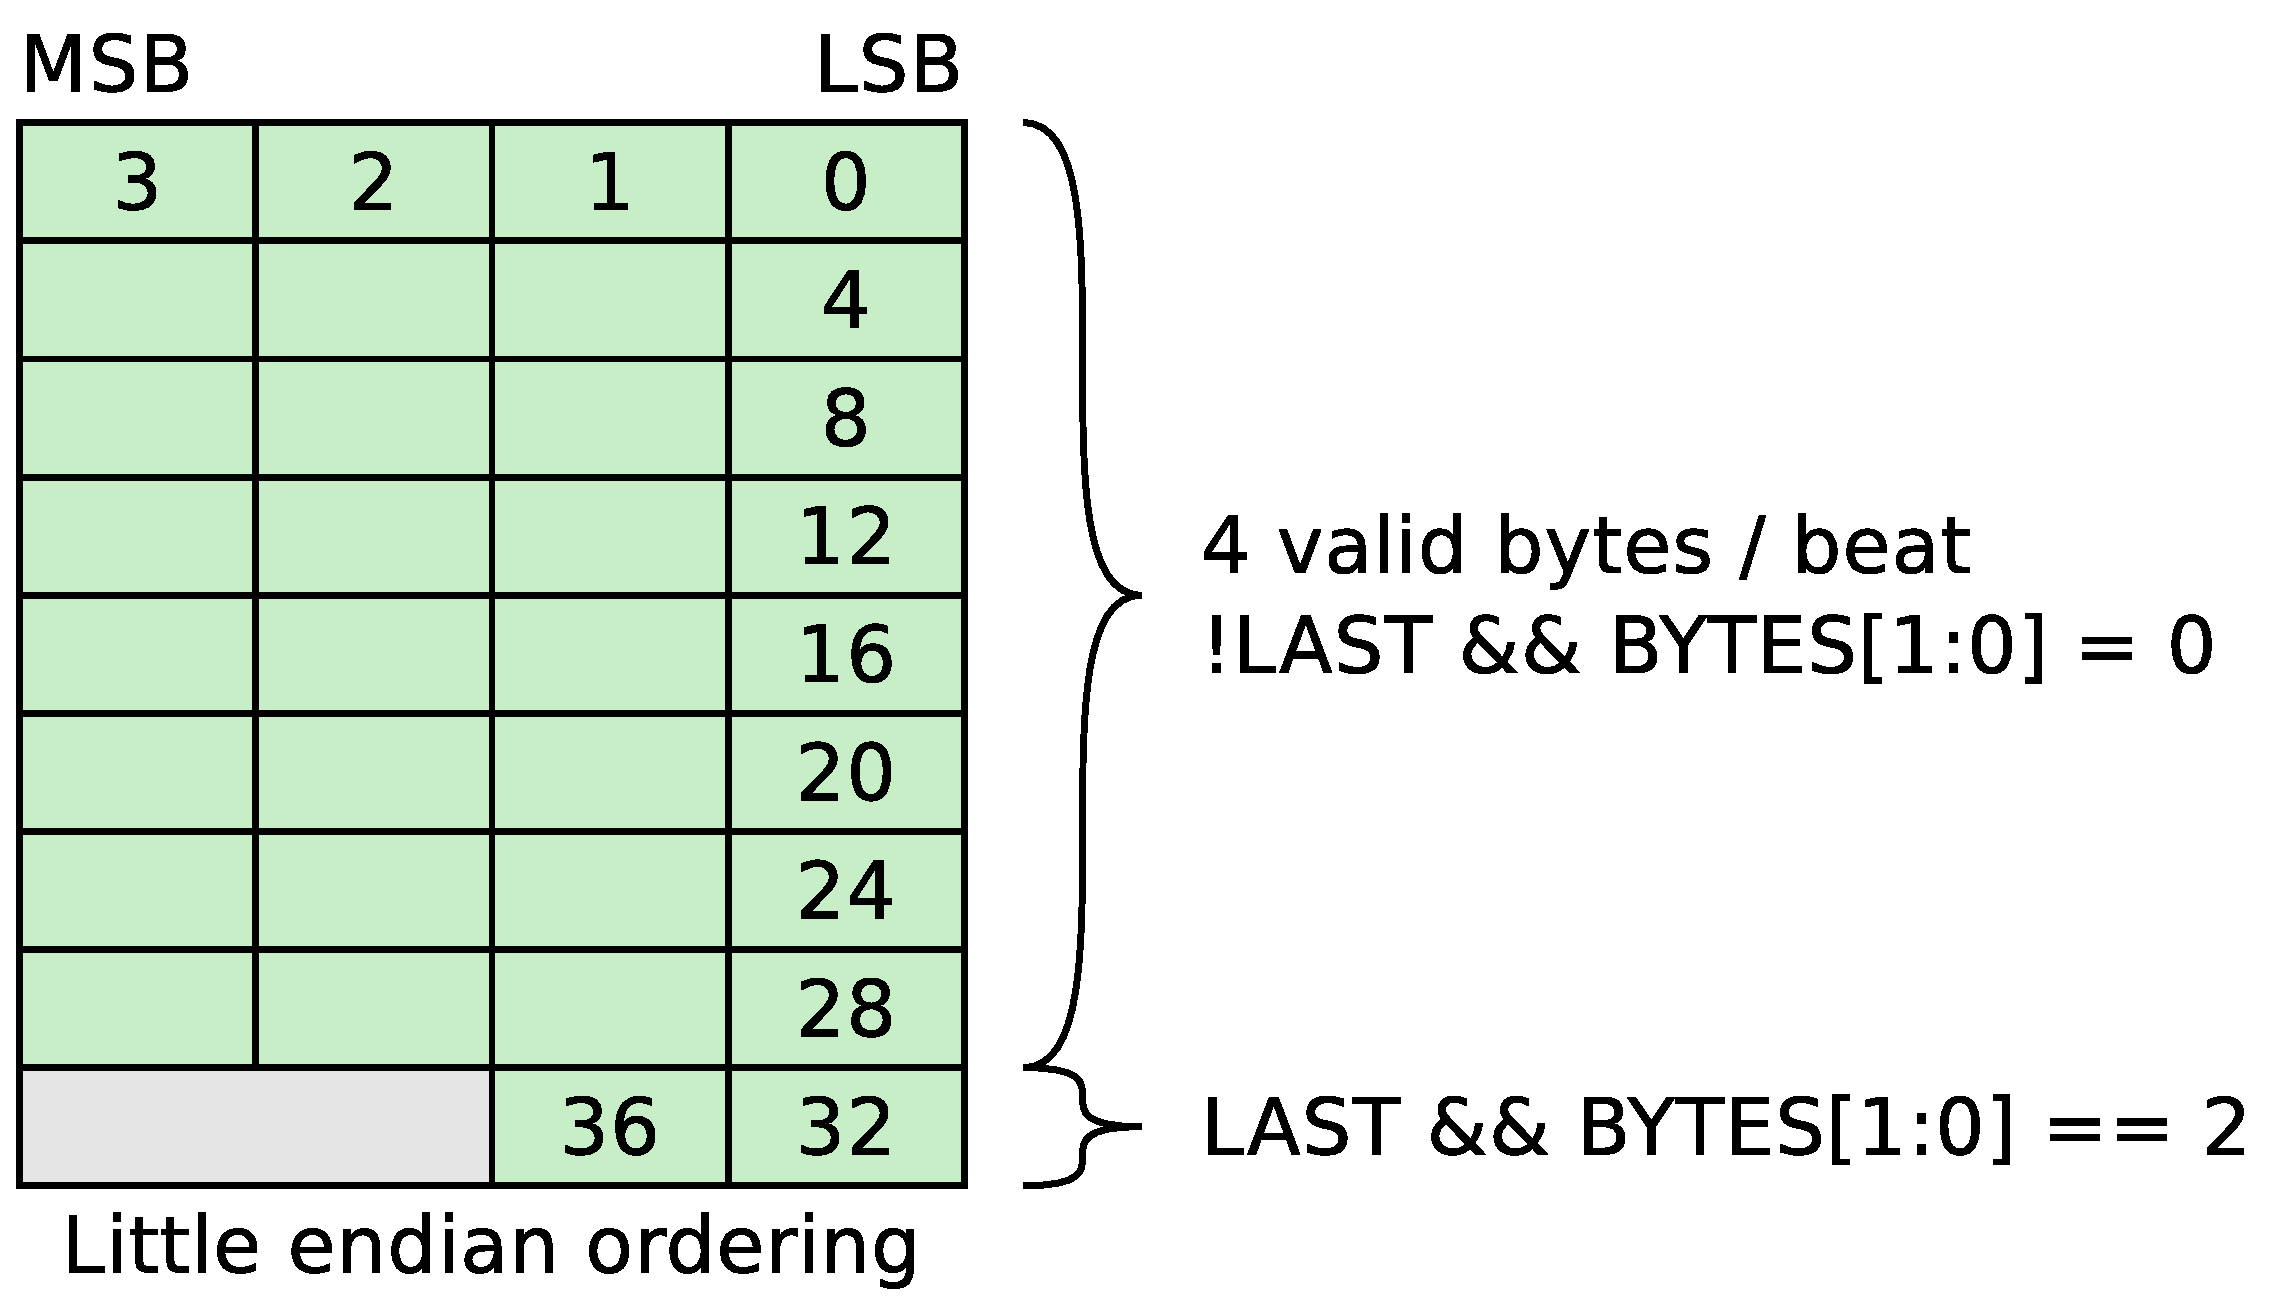
\includegraphics[width=2in]{little-endian.eps}}}
\end{center}
\end{slide}
%
%
%
%
\end{document}
%
%\fi
